% !TeX TS-program = xelatex

\documentclass[dvipsnames]{beamer}
\usetheme{metropolis}

\usepackage{multicol}

\usepackage{ragged2e} % who justifies the text
\usepackage{xecolor}
\usepackage{amsmath}
% \usefonttheme[onlymath]{serif} % change the math font

\usepackage{tabularx}
\usepackage{booktabs}
\usepackage[style=numeric,sorting=ynt]{biblatex}
\addbibresource{references.bib}
\usepackage[localise]{xepersian}

\settextfont{Vazir}
\setlatintextfont{Roboto}

% ---------------------------------------------------------------------------------
% Colors
% ---------------------------------------------------------------------------------
\definecolor{نارنجی}{rgb}{1.0, 0.31, 0.0}

% ---------------------------------------------------------------------------------
% Settings to force Beamer works with Xepersian and RTL typesetting
% ---------------------------------------------------------------------------------
% \raggedleft

% For right to left lists (itemize and enumerate)
\makeatletter
\newcommand{\لیست‌فارسی}{\raggedleft\rightskip\@totalleftmargin}
\makeatother
% Correct the bullet for RTL texts
\setbeamertemplate{itemize item}{\scriptsize\raise1.25pt%
	\hbox{\donotcoloroutermaths$\blacktriangleleft$}}

% To force beamer use numbering in captions
\setbeamertemplate{caption}[numbered]{}% Number float-like environments

\setbeamertemplate{footline}[frame number]
\setbeamertemplate{section in toc}[circle]
\setbeamertemplate{blocks}[rounded][shadow=true]
\setbeamercolor{block body}{bg=lightgray}
\setbeamercolor{headline}{bg=orange}
\setbeamersize{text margin left=1cm,text margin right=1cm}

\setbeamertemplate{headline}
{
	\begin{beamercolorbox}{section in head/foot}
		\vspace{2pt}\insertnavigation{\paperwidth}\vspace{2pt}
	\end{beamercolorbox}
}

% ---------------------------------------------------------------------------------
% To force beamer use numbering in captions
\setbeamertemplate{caption}[numbered]{}% Number float-like environments

\setbeamertemplate{footline}
{%
	\leavevmode%
	\hbox{%
		\begin{beamercolorbox}[wd=.333333\paperwidth,ht=2.25ex,dp=1ex,center]{author in head/foot}%
			\usebeamerfont{author in head/foot}\insertshortauthor%
		\end{beamercolorbox}%
		\begin{beamercolorbox}[wd=.333333\paperwidth,ht=2.25ex,dp=1ex,center]{title in head/foot}%
			\usebeamerfont{title in head/foot}\insertshorttitle%
		\end{beamercolorbox}%
		\begin{beamercolorbox}[wd=.333333\paperwidth,ht=2.25ex,dp=1ex,right]{date in head/foot}%
			\usebeamerfont{date in head/foot}\insertsection\hspace*{2em}
			\insertframenumber~ از \inserttotalframenumber{} \hspace*{2ex}%
		\end{beamercolorbox}
	}%
}
\setbeamertemplate{section in toc}[circle]
\setbeamertemplate{blocks}[rounded][shadow=true]
\setbeamercolor{block title}{bg=orange}
\setbeamercolor{block body}{bg=lightgray}
\setbeamersize{text margin left=1cm,text margin right=1cm}
\setbeamertemplate{frametitle continuation}{\insertcontinuationcount}

% ---------------------------------------------------------------------------------
\title{ارزیابی کارآیی انتها به انتها شبکه‌های توان پایین}
\subtitle{}
\author{پرهام الوانی}
\institute{%
	دانشکده مهندسی کامپیوتر\\
	دکتر مهدی راستی
}
\date{\today}
\titlegraphic{\vspace{4.5cm}\flushleft
\includegraphics[height=50pt]{images/logo}}

\begin{document}

\makeatletter

\setbeamertemplate{title}{%
	\linespread{1.0}%
	\inserttitle%
	\par%
	\vspace*{0.5em}
}
\setbeamertemplate{subtitle}{%
	\insertsubtitle%
	\par%
	\vspace*{0.5em}
}

\AtBeginSection[]
{%
	\begin{frame}{فهرست}
		\tableofcontents[currentsection]
	\end{frame}
	\begin{frame}
		\begin{center}
			\insertsectionnumber. \insertsection%
		\end{center}
		\usebeamertemplate*{title separator}
	\end{frame}
}

\makeatother


\begin{persian}
	% ------------------------------------------
	% Title frame (0)
	% ------------------------------------------
	{%
		\setbeamertemplate{footline}{}
		\begin{frame}
			\titlepage%
		\end{frame}
	}

	% -------------------------------------------------------------------------------
	\begin{frame}{فهرست}
		\tableofcontents[pausesections]
	\end{frame}

	% -------------------------------------------------------------------------------
	\section{شبکه‌های \متن‌لاتین{LoRa}}

	\begin{frame}
	  \begin{figure}
		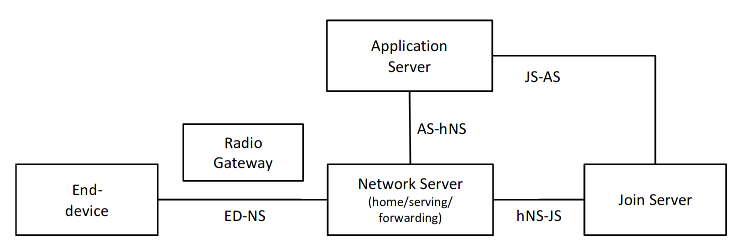
\includegraphics[width=\textwidth]{./images/nrm-home.png}
		\centering
		\caption{مدل مرجع شبکه \متن‌لاتین{LoRaWAN} - شبکه‌ی خانگی}
	  \end{figure}
	\end{frame}

	\begin{frame}
	  \begin{figure}
		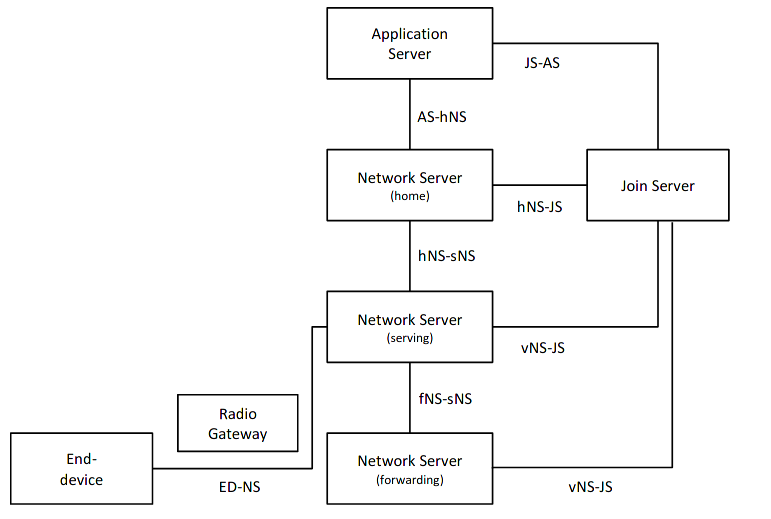
\includegraphics[width=\textwidth]{./images/nrm-roaming.png}
		\centering
		\caption{مدل مرجع شبکه \متن‌لاتین{LoRaWAN} - شبکه‌ی فراگرد}
	  \end{figure}
	\end{frame}

	\begin{frame}
	  \begin{figure}
		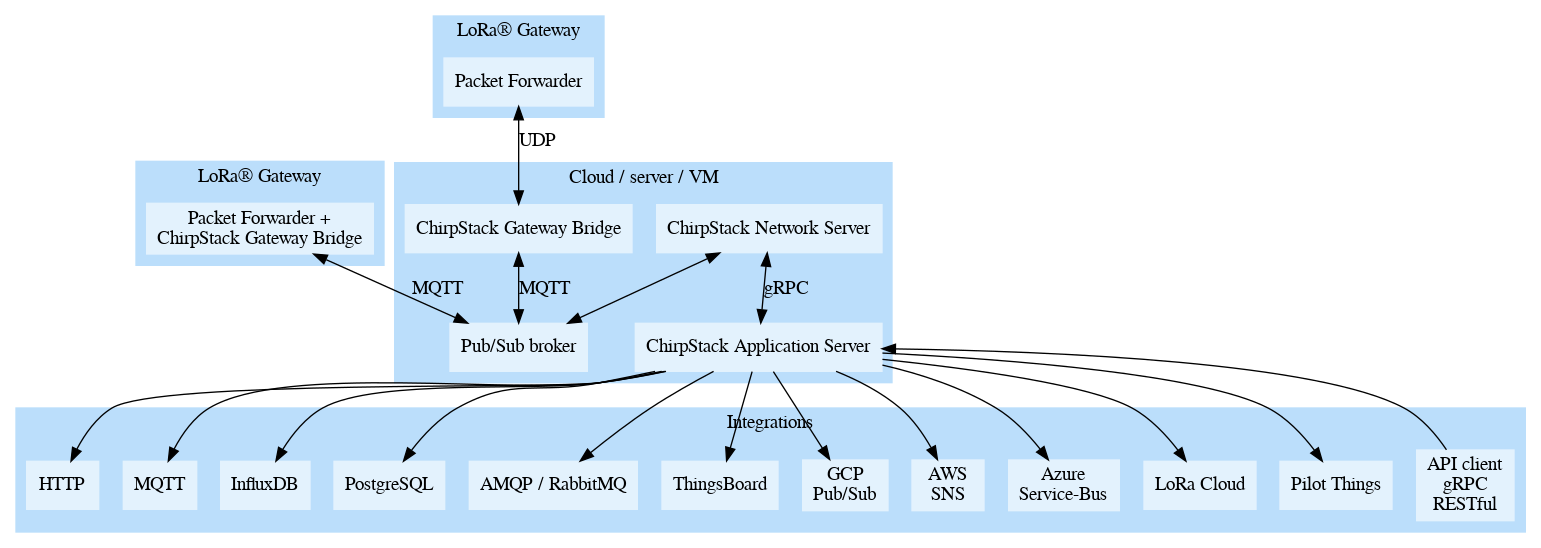
\includegraphics[width=\textwidth]{./images/chirpstack-architecture.png}
		\centering
		\caption{معماری \متن‌لاتین{LoRaWAN} سرور متن باز \متن‌لاتین{Chirpstack}}
	  \end{figure}
	\end{frame}

	\begin{frame}
	  کارگروه‌های مرتبط \متن‌لاتین{IETF}
	  \شروع{فقرات}
	  \لیست‌فارسی
	  \فقره \متن‌لاتین{A Semantic Definition Format for Data and Interactions of Things}
	  \فقره \متن‌لاتین{Concise Binary Object Representation Maintenance and Extensions}
	  \فقره \متن‌لاتین{Constrained RESTful Environments}
	  \فقره \متن‌لاتین{IPv6 over Low Power Wide-Area Networks}
	  \پایان{فقرات}
	\end{frame}

	\section{کارهای مرتبط}
	\begin{frame}[allowframebreaks]{}
		\fontsize{5pt}{6pt}\selectfont
		\begin{tabularx}{\textwidth}{|*{12}{X|}}
			\toprule
			مرجع &
			تحرک &
			پوشش &
			شبکه &
			لایه انتقال &
			لایه اپلیکشن &
			اندازه بسته &
			\متن‌لاتین{Coding Rate} &
			تاخیر &
			محیط &
			\متن‌لاتین{LoRa Mesh} &
			شبیه‌سازی \\
			\midrule
			\cite{sensors-18-00772-v3} &
			سیار &
			گزارش شده &
			\متن‌لاتین{LoRa} &
			ندارد &
			ندارد &
			گزارش شده &
			گزارش شده &
			گزارش نشده &
			باز &
			ندارد &
			واقعی / \متن‌لاتین{cloudRF} \\
			\midrule
			\cite{sensors-19-00007} &
			ثابت &
			گزارش شده &
			\متن‌لاتین{NB-IoT} &
			\متن‌لاتین{TCP / UDP} &
			\متن‌لاتین{MQTT / CoAP} &
			گزارش شده &
			گزارش نشده &
			گزارش شده &
			باز &
			ندارد &
			\متن‌لاتین{Ericsson inter. sim.} \\
			\midrule
			\cite{sensors-20-03061-v2} &
			ثابت &
			گزارش شده &
			\متن‌لاتین{LoRa} &
			ندارد &
			ندارد &
			گزارش شده &
			گزارش شده &
			گزارش شده &
			باز / بسته &
			ندارد &
			\متن‌لاتین{ns-3} \\
			\midrule
			\cite{sensors-20-00280-v2} &
			ثابت &
			گزارش شده &
			\متن‌لاتین{LoRa} &
			\متن‌لاتین{UDP ov IPv6} &
			\متن‌لاتین{CoAP} &
			گزارش شده &
			گزارش شده &
			گزارش شده &
			باز / بسته &
			ندارد &
			واقعی \\
			\midrule
			\cite{sensors-20-06721} &
			ثابت &
			گزارش شده &
			\متن‌لاتین{LoRa} &
			ندارد &
			ندارد &
			گزارش شده &
			گزارش شده &
			گزارش شده &
			بسته &
			ندارد &
			واقعی \\
			\midrule
			\cite{sustainability-12-08443} &
			متحرک &
			گزارش شده &
			\متن‌لاتین{LoRa \ NB-IoT} &
			\متن‌لاتین{UDP/TCP ov IPv6} &
			\متن‌لاتین{CoAP / ReST} &
			گزارش شده &
			گزارش شده &
			گزارش شده &
			باز &
			ندارد &
			واقعی \\
			\midrule
			\cite{Lee2018} &
			ثابت &
			گزارش شده &
			\متن‌لاتین{LoRa} &
			ندارد &
			ندارد &
			گزارش نشده &
			گزارش شده &
			گزارش شده &
			باز & / بسته
			دارد &
			واقعی \\
			\bottomrule
		\end{tabularx}
	\end{frame}

	\begin{frame}{\cite{sensors-18-03995}}
		\شروع{فقرات}
		\لیست‌فارسی
		\فقره مرور جامع مسائل و چالش‌های شبکه‌های \متن‌لاتین{LoRaWAN}
		\پایان{فقرات}
	\end{frame}

	\begin{frame}{\cite{sensors-18-00772-v3}}
		\شروع{فقرات}
		\لیست‌فارسی
		\فقره یک نود متحرک که پارامترهای ارسالش با زمان تغییر می‌کند.
		\فقره ناحیه‌های شهری، نیمه‌شهری و غیرشهری
		\فقره ارزیابی رادیویی بر پایه مدل انتشار \متن‌لاتین{Okumura-Hata} پیش از انجام ارزیابی عملیاتی
		\فقره نود متحرک برای بازه‌های زمانی ثابت می‌ماند تا تاثیر حرکت در پارامترها دیده شود.
		\فقره در انتها این پژوهش بیان می‌کند برای اجرای یک زیرساخت \متن‌لاتین{LoRaWAN} باید مصالحه‌ای بین کیفیت لینک، نرخ داده‌ی انتقالی و سیار بودن نود برقرار شود.
		\پایان{فقرات}
	\end{frame}

	\begin{frame}{\cite{sensors-19-00007}}
		\شروع{فقرات}
		\لیست‌فارسی
		\فقره ارزیابی بین \متن‌لاتین{MQTT} و \متن‌لاتین{CoAP} که به ترتیب بر بسترهای \متن‌لاتین{UDP} و \متن‌لاتین{TCP} فعالیت می‌کنند.
		\فقره شبکه زیرساخت \متن‌لاتین{NB-IoT} می‌باشد که با فعالیت روی باند دارای لایسنس و نبود \متن‌لاتین{duty-cycle} امکان اجرای \متن‌لاتین{tcp} را نیز فراهم می‌آورد.
		\فقره نشان می‌دهد \متن‌لاتین{MQTT} نسبت به \متن‌لاتین{CoAP} کارآیی کمتری در معیارهای تاخیر، پوشش و ظرفیت سیستم دارد.
		\پایان{فقرات}
	\end{frame}

	\begin{frame}{\cite{sensors-20-03061-v2}}
		\شروع{فقرات}
		\لیست‌فارسی
		\فقره \رنگ‌متن{نارنجی}{جداسازی پیام‌های دورسنجی از اخطارها} به وسیله‌ی شبه عمود بودن \متن‌لاتین{SF}ها در شبکه‌های \متن‌لاتین{LoRaWAN}.
		\فقره استفاده از دو استراتژی برای تخصیص \متن‌لاتین{SF}های متمایز برای داده‌های اخطاری و داده‌های دورسنجی
		\فقره آزمایش عملی این پژوهش به دلیل نیاز به تعداد بالای نود و نیاز به تغییر رویه تخصص \متن‌لاتین{SF}ها امکان‌پذیر نیست.
		\پایان{فقرات}
	\end{frame}

	\begin{frame}{\cite{sensors-20-00280-v2}}
		\شروع{فقرات}
		\لیست‌فارسی
		\فقره پیاده‌سازی الگوریتم \متن‌لاتین{Static Context Header Compression (SCHC)} برای \متن‌لاتین{IPv6} و استفاده از آن برای انتقال \متن‌لاتین{CoAP} بر پایه \متن‌لاتین{UDP}
		\فقره منابع مصرفی در جهت استفاده از \متن‌لاتین{IPv6} نسبت به سود حاصل از آن بسیار کم است. در مقابل کارایی انرژی و داده در \متن‌لاتین{fragmentation} کم است.
		\فقره زمانی یک نود بین \متن‌لاتین{gateway}ها جابجا می‌شود در صورت لزوم پروسه پیوستن به \متن‌لاتین{NS} را انجام می‌دهد. در صورت استفاده از یک آدرس \متن‌لاتین{IPv6} ثابت اتصال تضمین می‌شود.
		\فقره برای استفاده از قطعه‌بندی \متن‌لاتین{IETF} نیاز است که ترتیب بسته‌ها حفظ شود.
		\فقره در نظر گرفتن نودهای متحرک و سناریوهای انتها به انتها چیزی که در این پژوهش به آن پرداخته نشده است.
		\پایان{فقرات}
	\end{frame}

	\begin{frame}{\cite{sensors-20-06721}}
		\شروع{فقرات}
		\لیست‌فارسی
		\فقره تجربه بیش از دو سال مدیریت و نگهداری شبکه‌های سنسورهای داخلی مبتنی بر \متن‌لاتین{LoRa}
		\فقره از دست رفتن بسته‌ها به جز در انتقال در \متن‌لاتین{Backend} هم رخ می‌دهد. نرخ ارسال سنسورها ۱۵ دقیقه می‌باشد.
		\فقره مقالات بسیاری را بر پایه این تجربه به چاپ رسانده‌اند.
		\فقره منظور از شبکه \متن‌لاتین{Backend} زیرساخت ارتباط میان \متن‌لاتین{NS} و سرور پلتفرم می‌باشد.
		\فقره این بازه‌های از دست رفتن بیش از ۵۰ درصد بسته‌ها در \متن‌لاتین{Backend} به صورت دوره‌های ۱.۵ ماه رخ می‌دادند. این پژوهش به بررسی بیشتر این موضوع نپرداخته است.
		\فقره استفاده از فعال‌سازی \متن‌لاتین{OTAA}
		\پایان{فقرات}
	\end{frame}

	\begin{frame}{\cite{sensors-20-02078}}
		\شروع{فقرات}
		\لیست‌فارسی
		\فقره کارهای زیادی برای کشاورزی دقیق و با مصرف باطری کم پیشنهاد شده‌اند اما تعداد کمی از آن‌ها در عمل تست شده‌اند.
		\فقره این پژوهش قصد دارد مصرف انرژی قسمت‌های مختلف را در شرایط واقعی محاسبه و کاهش دهد.
		\فقره زمانی که داده‌ی زیادی برای ارسال موجود نیست مانند سنسورهای کشاورزی، استفاده از \متن‌لاتین{LoRa} گزینه خوبی است.
		\فقره پوشش \متن‌لاتین{LTE} در نواحی غیرشهری و کشاورزی کافی نیست بنابراین استفاده از \متن‌لاتین{NB-IoT} گزینه خوبی نیست.
		\فقره محاسبه نرخ منطقی ۳۰ دقیقه برای ارسال داده‌ها
		\پایان{فقرات}
	\end{frame}

	\begin{frame}{\cite{sensors-21-01924-v2}}
		\شروع{فقرات}
		\لیست‌فارسی
		\فقره ارائه یک روش کاهش حجم داده مبتنی بر حذف داده‌های تکراری
		\فقره این روش به صورت عام بوده و می‌توان آن را با روش \متن‌لاتین{SCHC} ترکیب کرد.
		\پایان{فقرات}
	\end{frame}

	\begin{frame}{\cite{sustainability-12-08443},\cite{Santa2020}}
		\شروع{فقرات}
		\لیست‌فارسی
		\فقره پیاده‌سازی یک \متن‌لاتین{OBU} برای وسایل حمل و نقل نوظهور (مانند دوچرخه یا اسکوترهای برقی)
		\فقره استفاده از \متن‌لاتین{NB-IoT} و \متن‌لاتین{LoRaWAN} برای ارتباط \متن‌لاتین{OBU}ها
		\فقره تکنولوژی‌های ارتباطی سلولی برای ارتباط‌های حیاتی حفظ می‌شوند و داده‌های مانتورینگ و \نقاط‌خ از طریق شبکه‌های \متن‌لاتین{LPWAN} ارسال می‌شوند.
		\فقره به صورت عملی از زیرساخت \متن‌لاتین{Vodafone} برای \متن‌لاتین{NB-IoT} استفاده کرده‌اند.
		\پایان{فقرات}
	\end{frame}

	\begin{frame}{\cite{Marahatta2021}}
		\شروع{فقرات}
		\لیست‌فارسی
		\فقره ارزیابی شبکه‌های \متن‌لاتین{LoRaWAN} برای کنترل مصرف انرژی در مناطق دورافتاده
		\فقره پیاده‌سازی مفهوم \رنگ‌متن{نارنجی}{\متن‌لاتین{LoRa Mesh}} که در آن هر نود به عنوان تکرارکننده برای نودهای همسایه خود عمل می‌کند.
		\فقره ارزیابی بر پایه شبیه‌سازی \متن‌لاتین{NS2} صورت پذیرفته است. برای شبیه‌سازی از مناطق شهری و غیرشهری استفاده شده است و در صورت نیاز شبکه به زیرشبکه‌هایی شکسته شده است.
		\فقره معرفی معیار حداقل زمان لازم برای استخراج موفقیت آمیز داده
		\پایان{فقرات}
	\end{frame}

	\begin{frame}{\cite{Famaey2018}}
		\شروع{فقرات}
		\لیست‌فارسی
		\فقره در نظر گرفتن یک شبکه یکپارچه مبتنی بر تکنولوژی‌های ارتباطی متنوع
		\فقره تعریف اپراتور مجازی شبکه اینترنت اشیا که سطح انتزاعی برای برنامه‌های کاربردی از انواع مختلف شبکه‌ها فراهم می‌آورد.
		\فقره استفاده از \متن‌لاتین{IPv6} در لایه شبکه و از \متن‌لاتین{CoAP} در لایه کاربرد
		\پایان{فقرات}
	\end{frame}

	\begin{frame}{\cite{Islam2021}}
		\شروع{فقرات}
		\لیست‌فارسی
		\فقره مساله استفاده از \متن‌لاتین{UAV}ها و ارتباطات \متن‌لاتین{LoRaWAN} و ماهواره‌ای در کشاورزی
		\فقره مساله محدودیت ارتباط در این حوزه به قدر کافی مورد توجه قرار نگرفته است.
		\فقره بررسی محدودیت‌های ارتباط در \متن‌لاتین{UAV}ها
		\فقره پیاده‌سازی مفهوم \رنگ‌متن{نارنجی}{\متن‌لاتین{Meshed LoRaWAN Gateway}} که در آن:
		\شروع{فقرات}
		\لیست‌فارسی
		\فقره کارآیی و قابلیت بسیار پایین است.
		\فقره نیاز به نگهداری از راه دور برای دروازه‌ها وجود دارد.
		\فقره نیاز به پردازش لبه در دروازه‌ها وجود دارد.
		\پایان{فقرات}
		\پایان{فقرات}
	\end{frame}

	\begin{frame}{\cite{Lee2021}}
		\شروع{فقرات}
		\لیست‌فارسی
		\فقره از جمله مقالاتی است که در بهبود لایه \متن‌لاتین{MAC} برای بهبود شبکه‌های \متن‌لاتین{LoRa} در مقیاس بزرگ کار کرده است.
		\فقره ارسال گروهی \متن‌لاتین{ACK} برای پیام‌های دارای تاییدیه \متن‌لاتین{LoRaWAN} در این ساختار جدید لایه \متن‌لاتین{MAC} مورد بررسی قرار گرفته است.
		\فقره در این پیاده‌سازی جدید از \متن‌لاتین{Beacon}ها برای همگام‌سازی استفاده میشود تا ساختار \متن‌لاتین{Frame} مشخص شود.
		\فقره در هر \متن‌لاتین{Frame} امکان ارسال \متن‌لاتین{uplink} و \متن‌لاتین{downlink} در بازه‌های مشخص وجود دارد.
		\پایان{فقرات}
	\end{frame}

	\begin{frame}[allowframebreaks]{\cite{Lee2018}}
		\شروع{فقرات}
		\لیست‌فارسی
		\فقره پیاده‌سازی ۱۹ نود شبکه‌ی \متن‌لاتین{Mesh LoRaWAN} در محیط دانشگاه با ارسال داده‌ها در بازه‌های یک دقیقه‌ای.
		\فقره اولین کاری است که تجربه واقعی در پیاده‌سازی \متن‌لاتین{Mesh LoRaWAN} داشته است و در آن بیان می‌شود با این روش نیاز به افرایش تعداد \متن‌لاتین{Gateway}ها از بین می‌رود.
		\فقره نویسندگان معتقد هستند که استفاده از \متن‌لاتین{ALOHA} توانایی \متن‌لاتین{LoRa} در هندل کردن تعداد زیادی از اشیا را از بین برده است.
		\فقره سیستم طراحی شده در این پژوهش به جای \متن‌لاتین{LoRaWAN} بر پایه لایه‌ی فیزیکی \متن‌لاتین{LoRa} می‌باشد.
		\فقره نودها به صورت خودمختار برای انتخاب پدر خود در زمان پیوستن به شبکه‌ی \متن‌لاتین{Mesh} تصمیم می‌گیرند، آن‌ها برای این امر از پارامترهای پیام‌های داده‌ای یا \متن‌لاتین{Beacon}های نودهای متصل به شکبه، که به آن‌ها می‌رسد، استفاده می‌کنند.
		\فقره در این ساختار هر نود لیستی از فرزندان خود نگهداری کرده و آن را در اختیار \متن‌لاتین{‌Gateway} هم قرار می‌دهد.
		\فقره این شبکه برای ارتباطات بین نودها بهینه نشده است و بیشتر هدف آن ارتباط میان \متن‌لاتین{Gateway} و نودها می‌باشد.
		\فقره این پژوهش در مورد مقدار بهینه پارامترهای \متن‌لاتین{RSSI} و \نقاط‌خ صحبت می‌کند و بیان می‌کند که برای رسیدن به این مقدارهای بهینه نیاز به افزایش تعداد \متن‌لاتین{Gateway}ها یا استفاده از شبکه‌ی \متن‌لاتین{Mesh} می‌باشد.
		\فقره در این پروژه \متن‌لاتین{Gateway} برای دریافت داده‌ها به نودها درخواست می‌دهد و در مورد ارسال خودکار داده‌ها توسط اشیا که می‌تواند منجر به \متن‌لاتین{Collusion} شود بحث نشده است.
		\فقره در نظر نگرفتن کلاس‌های کاری و توان مصرفی شبکه‌ی \متن‌لاتین{LoRa}
		\پایان{فقرات}
	\end{frame}

	\section{گپ پژوهشی}

	\begin{frame}
		\شروع{فقرات}
		\لیست‌فارسی
		\فقره لایه اشیا
		\شروع{فقرات}
		\لیست‌فارسی
		\فقره پیاده‌سازی \متن‌لاتین{LoRa Mesh} به صورت عملی و بررسی چالش‌های زمان‌بندی و \نقاط‌خ مانند \مرجع{Lee2018}
		\فقره مساله‌ی مکان‌یابی در فضای بسته با استفاده از \متن‌لاتین{LoRa} یا \متن‌لاتین{WiFi} یا هر دو
		\فقره استفاده از الگوریتم‌های نوبت‌دهی متفاوت از \متن‌لاتین{unslotted ALOHA} مانند \مرجع{Lee2021}
		\فقره تخصیص منابع مخابراطی مانند \متن‌لاتین{SF}ها و \نقاط‌خ
		\فقره انتخاب تکنولوژی مناسب ارتباطی به صورت خودکار توسط شی
		\فقره استفاده از آنتن‌های جهت‌دار برای کاهش نویز در شبکه‌های با چگالی بالا
		\پایان{فقرات}
		\پایان{فقرات}
	\end{frame}

	\begin{frame}
		\شروع{فقرات}
		\لیست‌فارسی
		\فقره لایه دسترسی
		\شروع{فقرات}
		\لیست‌فارسی
		\فقره در نظر گرفتن شی متحرک با جابجایی میان \متن‌لاتین{Gateway}ها و انجام رویه‌ی \متن‌لاتین{Roaming} (در دوچرخه‌های هوشمند و \نقاط‌خ کاربرد دارد)
		\فقره در نظر گرفتن کلاس‌های مختلف اشیا در شبکه‌های \متن‌لاتین{LoRaWAN}
		\فقره در نظر گرفتن استفاده مشترک در شبکه‌های \متن‌لاتین{WiFi} و انجام رویه \متن‌لاتین{Handover}
		\فقره در نظر گرفتن سیستم انتها به انتها مبتنی بر \متن‌لاتین{IPv6}
		\فقره در نظر گرفتن نودهای عملگر
		\فقره در نظر گرفتن الویت و کیفیت سرویس
		\پایان{فقرات}
		\پایان{فقرات}
	\end{frame}

	\begin{frame}
	  \شروع{فقرات}
	  \لیست‌فارسی
	  \فقره لایه هسته
	  \فقره لایه هسته خود می‌تواند شامل پلتفرم اینترنت اشیا و برنامه‌های کاربردی باشد.
	  \شروع{فقرات}
	  \لیست‌فارسی
	  \فقره پردازش داده‌های شبکه‌های \متن‌لاتین{LoRaWAN} و \متن‌لاتین{WiFi} بر پایه \متن‌لاتین{IPv6}
	  \فقره مساله چگونگی کد شدن داده‌ها (\متن‌لاتین{SenML})
	  \فقره مساله مدل داده‌ای سنسورها (\متن‌لاتین{OneDM})
	  \فقره یکسان‌سازی مدل داده‌ای و چگونگی کد شدن در سطح پلتفرم و برنامه‌های کاربردی و مساله پیدا کردن خودکار اشیا
	  \فقره استفاده از الگوریتم‌های یادگیری ماشین به صورت توزیع شده (\متن‌لاتین{Federated Learning})
	  \پایان{فقرات}
	  \پایان{فقرات}
	\end{frame}

	\section{مسائل پیشنهادی}

	\begin{frame}{کاربرد}
	  \شروع{فقرات}
	  \لیست‌فارسی
	  \فقره محوطه دانشگاه هوشمند - \متن‌لاتین{Smart Campus}
	  \فقره کشاورزی هوشمند - \متن‌لاتین{Smart Farming}
	  \پایان{فقرات}
	\end{frame}

	\begin{frame}{مساله ۱}
	  ارزیابی کارآیی \متن‌لاتین{Backbone} مبتنی بر \متن‌لاتین{IP} شبکه‌های \متن‌لاتین{LoRaWAN}
	  \شروع{فقرات}
	  \لیست‌فارسی
	  \فقره نرخ ارسال داده‌ها
	  \فقره پیاده‌سازی لینک \متن‌لاتین{AS-hNS}
	  \پایان{فقرات}
	\end{frame}

	\begin{frame}{مساله ۲}
	  در نظر گرفتن تاثیر رویه ارسال و نرخ ارسال داده‌ها برای کارآیی شبکه‌های \متن‌لاتین{LoRaWAN} و منابع مصرفی اشیا در کنار شبکه‌ی هسته
	  \شروع{فقرات}
	  \لیست‌فارسی
	  \فقره اشیا می‌توانند به سه روش کلی زیر ارسال داده داشته باشند که هر یک نیازمندی‌های کیفیت سرویس خاص خود را ایجاد می‌کند.
	  \شروع{فقرات}
	  \لیست‌فارسی
	  \فقره \متن‌لاتین{Periodic}
	  \فقره \متن‌لاتین{Self Trigger}
	  \فقره \متن‌لاتین{Trigger by Event}
	  \پایان{فقرات}
	  \فقره شبکه‌ی هسته می‌بایست بین بسته‌های دریافتی بسته‌های با الویت بیشتر را پردازش کند و الگوریتم‌زمان‌بندی داشته باشد.
	  \پایان{فقرات}
	\end{frame}

	\begin{frame}{مساله ۳}
	  پیاده‌سازی یک پلتفرم با قابلیت شناسایی خودکار داده‌ها و اشیا
	  \شروع{فقرات}
	  \لیست‌فارسی
	  \فقره استفاده از مدل داده‌ای \متن‌لاتین{Semantic Definition Format}
	  \فقره
	  \پایان{فقرات}
	\end{frame}

	\begin{frame}{پروژه‌های کارشناسی}
	  \شروع{فقرات}
	  \لیست‌فارسی
	  \فقره پیاده‌سازی کتابخانه‌ی \متن‌لاتین{SenML} با زبان \متن‌لاتین{C} یا \متن‌لاتین{C++} و \متن‌لاتین{CBOR}
	  \پایان{فقرات}
	\end{frame}

	% -------------------------------------------------------------------------------
	\begin{frame}[allowframebreaks]{مراجع}
		\begin{latin}
			\printbibliography[title=مراجع]
		\end{latin}
	\end{frame}

\end{persian}
\end{document}
